\capitulo{3}{Conceptos teóricos}

%En aquellos proyectos que necesiten para su comprensión y desarrollo de unos conceptos teóricos de una determinada materia o de un determinado dominio de conocimiento, debe existir un apartado que sintetice dichos conceptos.

Para la comprensión de este proyecto será necesario la compresión de algunos conceptos teóricos que introduciré en este apartado:

\begin{itemize}
	\item Inteligencia artificial
	\item Aprendizaje automático
	\item Aprendizaje supervisado y no supervisado
	\item Clasificación
	\item Reconocimiento de patrones
	\item Segmentación
	\item Binarización
	\item \textit{Thresholding}
	\item Descriptores visuales
	%\item Maquinas de vector soporte
	\item \textit{Bag of Words}
	\item Detección de objetos
	\item mAP
	\item YOLO
\end{itemize}


\section{Inteligencia artificial}

Inteligencia artificial, que comúnmente aparece como las siglas IA o AI del ingles, consiste en otorgar a las máquinas la capacidad de realizar acciones que habitualmente son realizadas por humanos, imitando la inteligencia cognitiva humana \cite{alanturing:ai}. Esta podría ser una posible definición de Inteligencia artificial, pero existen multitud \cite{russell1995modern}. Algunos posibles ejemplos conocidos por todos en los que se aplica la IA son el coche autónomo, videojuegos, asistentes personales, reconocimiento facial en imágenes.

\section{Apredizaje automático}

Apredizaje automático, o en ingles \textit{machine learning}, es un campo de la informática cuyo objetivo es dar a los computadores la capacidad de aprender sin explícitamente haber sido programados\cite{wiki:machinelearning}. Por lo tanto, se encarga de construir modelos para problemas en los que un algoritmo programado no puede conseguir buenos resultados o es muy complejo hacer que lo sean.



\section{Aprendizaje supervisado y no supervisado}

En esta sección vamos a distinguir entre aprendizaje supervisado y no supervisado, ambas técnicas pertenecientes al campo de la informática \textit{machine learning}.

Aprendizaje supervisado es una técnica que consiste en la inferencia de una función partiendo de un conjunto de datos de entrenamiento etiquetado \cite{wiki:supervisedLearning}. Para tareas de clasificación o regresión. Es decir, para tareas en las que el resultado deseado sea obtener una variable que nos informe a que clase pertenece una determinada instancia, lo cual es un valor discreto, o para tareas en las que se desea obtener un valor continuo. Dos posibles ejemplos, a modo de aclaración,  podrían ser: la clasificación de \textit{emails} en \textit{spam} o \textit{no spam} y la predicción del valor de un inmueble.

En cuanto al otro tipo de aprendizaje, el aprendizaje no supervisado consiste en la obtención de la estructura oculta en los datos. Pero al contrario que en el aprendizaje supervisado, partiendo de un conjunto de datos sin etiquetar, es decir, datos para los cuales no poseemos su valor deseado\cite{wiki:unsupervisedLearning}. Un posible ejemplo  de la utilización de este tipo de aprendizaje podría ser la categorización de clientes en varios grupos con fines comerciales.

\section{Clasificación}

Clasificación es la tarea de identificar, entre un conjunto de  categorías o clases\footnote{Se entiende por clase a cada uno de los tipos de instancia que se desea clasificar. Por ejemplo, en un problema en el que deseemos clasificar imágenes como personas y perros. Las clases serán: persona y perro.}, a que categoría o clase pertenece una determinada instancia.

En el caso de este proyecto, estamos tratando de clasificar los distintos tipos de fitolitos. Por lo tanto tendremos tantas clases como tipos de fitolitos, además, de una clase que indica    que no existe fitolito, es decir, negativos.

\section{Reconocimiento de patrones}

El reconocimiento de patrones consiste en la extracción de propiedades similares entre las distintas instancias de una clase \cite{wiki:patternrecognition}. De manera que podamos identificar un determinado objeto en función de los patrones que contiene este. Este concepto, como podemos observar, está íntimamente relacionado con el concepto de clasificación y \textit{machine larning}.

\section{Segmentación}

La segmentación en el campo de la visión artificial, como se indica en la wikipedia, consiste en subdividir una imagen en varios pixeles u objetos. \cite{wiki:segmentation}
Cuando segmentamos una imagen, lo que pretendemos hacer es cambiar su representación para poder obtener de esta una mayor utilidad o cantidad de información.

En nuestro caso, segmentamos la imagen para eliminar el fondo de ella y obtener así una imagen con solo su parte delantera. De esta manera, eliminamos el ruido que existe en la imagen y, a su vez, la simplificamos reteniendo la parte de la imagen en la que se encuentran los objetos que nos interesan.

Posteriormente a ese paso, nos interesa, como es obvio, dividir la parte delantera de la imagen resultante en objetos. De este modo, obtendremos cada uno de los objetos por separado de forma idónea.

\section{Binarización}

La binarización de una imagen consiste en la simplificación de los valores de cada pixel a 2 posibles valores, blanco o negro, representando el fondo y el frente de la imagen cada uno de ellos. Esta técnica nos permite conservar únicamente la información que nos interesa, eliminando el resto.

\section{Thresholding}

Es el método mas simple para la segmentación de una imagen, pudiendose utilizar para la binarización de una imagen, como es nuestro caso. Consiste en reemplazar los píxeles por debajo de una determinada constante a píxeles negros, y los que se encuentran por encima a píxeles blancos o viceversa.

Existen distintas maneras de llevar a cabo este proceso, siendo uno de lo más conocidos el método de Otsu. \cite{wiki:otsu}

\section{Descriptores visuales}

Los descriptores visuales, o descriptores de características, son descripciones de las características visuales de los contenidos en imágenes o videos, en nuestro caso de imágenes, con el proposito de la detección de objetos \cite{wiki:visualdescriptor}. El objetivo de los descriptores visuales es obtener la información que resulta significativa, eliminando a su vez la que no lo es. Así, utilizaremos la información que el descriptor nos proporciona para detectar los objetos que nos interesan en una imagen. Algunos ejemplos de características son la forma, el color o la textura.

Como se puede imaginar, obtener las características a mano es una tarea complicada y que usualmente no funciona correctamente. Por ello, utilizamos un método de extracción automática de características como es \textit{Histogram of Oriented Gradients}, el cual se basa en los gradientes de la imagen para detectar los distintos objetos que se encuentran en la imagen \cite{wiki:hog}.

\begin{comment}
\section{Máquinas de vectores soporte}

Las máquinas de vectores soporte, o SVM, son modelos de aprendizaje supervisados utilizados para tareas de clasificación o de regresión \cite{wiki:svm}. En nuestro caso este modelo se ve usado para tareas de clasificación, puesto que es lo que nos concierne en nuestra problemática.

Para que nuestra SVM sea capaz de clasificar los objetos, le proveemos de un conjunto de entrenamiento compuesto por positivos y negativos, es decir, ejemplos de los objetos que nos interesan y otros objetos, respectivamente. A partir de esta información nuestra SVM será capaz de clasificar nuevos ejemplos en las categorías pertinentes.
\end{comment}

\section{\textit{Bag of Words}}

\textit{Bag of Words} (BoW), o en español bolsa de palabras, es una técnica comúnmente utilizada en la clasificación de documentos \cite{wiki:bowmodel}. En la que se describe un texto mediante el conjunto de palabras que componen dicho texto.

Pero esta técnica también ha sido aplicada al reconocimiento de objetos en imágenes. Siendo, la técnica que mejores resultados conseguía, hasta la llegada del \textit{Deep Learning}. En este caso, se tratan las características de una imagen como palabras. 

\section{Reconocimiento de objetos contra Detección de objetos}

Antes de abordar el siguiente concepto, debemos de comprender la diferencia entre el término reconocimiento de objetos y detección de objetos.

Reconocimiento de objetos es el termino utilizado cuando se desea detectar todos los objetos para los que ha sido entrenado el clasificador. Proporcionándonos el tipo de objeto y las coordenadas de la caja que rodea ese objeto. E, incluso en algunos casos, las probabilidades de que ese objeto sea un verdadero positivo o un falso positivo.

En cuanto a la detección de objetos, en este solo se desea obtener si es objeto o no es objeto. Simplificando el problema anterior, de manera que, pasamos de un problema multiclase a un problema con dos clases. Objeto o no objeto.

\section{Media promedio de precisión (\textit{mAP})}

La media promedio de precisión, en ingles \textit{mean average precision} (\textit{mAP}), es comúnmente utilizada como una medida de evaluación de la precisión en la detección de objetos. %COMPLETAR

%\section{IOU}

%\section{VOc}?

%\section{Redes neuronales convolucionales}

%\section{Deep learning}

\section{\textit{YOLO}}

\textit{YOLO}, o \textit{You Only Look Once}, es una aproximación innovadora en la detección de objetos, considerándose actualmente el estado del arte en esta materia, junto a \textit{Faster RCNN}\footnote{Faster RCNN es un detector de objetos en tiempo real con una precisión similar a la última versión de \textit{YOLO}, pero con menor rendimiento en tiempos que \textit{este}}. Tratando de crear una arquitectura muy rápida pero, a su vez, siendo capaz de soportar un número de clases mayor a 9000 \cite{yolov2}.

\subsection{Versiones}

\textit{YOLO}, actualmente, tiene dos versiones. Y, en cada una de estas versiones, se ha desarrollado una versión pequeña y una normal. En la primera versión de \textit{YOLO} se consiguió llegar a resultados muy positivos, como la capacidad de procesar 45 imágenes por segundo con una precisión de 63.4 \textit{mAP}. Y, con la versión pequeña de este, se llegaron a procesar 155 imágenes por segundo con una precisión de 52.7 \textit{mAP}\cite{yolo}. Precisiones muy positivas, pero que todavía no estaban a la altura del estado del arte a nivel de precisión.

En la segunda versión, se considera a \textit{YOLO} como el estado del arte, junto a \textit{Faster RCNN}. En esta versión, \textit{YOLO} consigue llegar a una precisión de 76,8 \textit{mAP}, procesando 67 imágenes por segundo, y 78,6 \textit{mAP}, procesando 40 imágenes por segundo. Lo cual, supera a \textit{Faster RCNN} en precisión y rapidez, siendo esta última ampliamente superada \cite{yolov2}.\footnote{\textit{Faster RCNN} consigue clasificar una 1 imágenes cada 2 segundos. En cambio, \textit{YOLO} es capaz de procesar 40 imágenes.}

\subsection{Característica diferenciadora de \textit{YOLO}}

\textit{YOLO} otorga un enfoque distinto respecto a sus competidores. Mientras que en otros casos, como \textit{Faster RCNN}, se separan las distintas etapas del procesado de una imagen. \textit{YOLO}, he de aquí su nombre, solo necesita de un único <<vistazo>> para predecir la imagen y obtener las coordenadas, o cajas que rodean a cada uno de los objetos predichos \cite{yolo}.

Por supuesto, esta perspectiva no es tan simple como un giro en el enfoque. Sino que, además, implementa otras características, como la normalización en lotes o la obtención automática del tamaño de las cajas, que la permiten ser la mejor aproximación actual en este campo \cite{yolov2}.

Podemos ver una comparativa entre los mejores detectores de objetos actuales con \textit{YOLO} en la figura \ref{fig:3.2.13}. Indicando para cada uno de ellos la precisión y la capacidad de procesamiento de imágenes, en las unidades de media promedio de precisión e imágenes por segundo, respectivamente.

\begin{figure}[h]
\centering
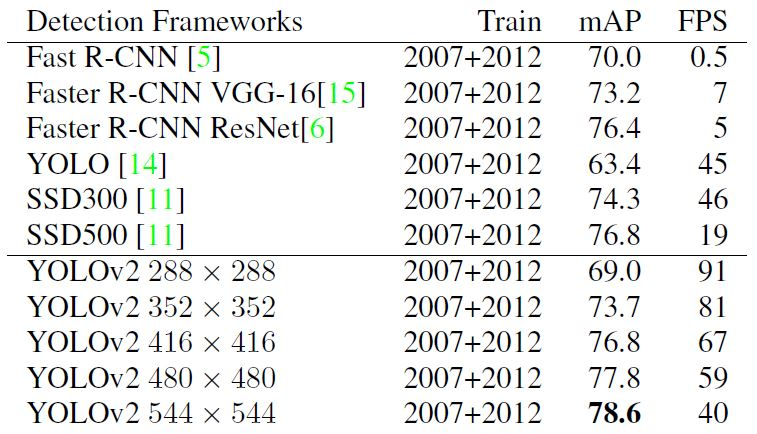
\includegraphics[width=0.5\textwidth]{comparativa_yolo}
\caption{Comparativa entre los distintos sistemas de detección de objetos sobre el mismo conjunto de entrenamiento y sobre la misma configuración \cite{yolov2}.}
\label{fig:3.2.13}
\end{figure}


% Por aclarar más cosas